%%%%%%%%%%%%%%%%%%%%%%%%%%%%%%%%%%%%
%%                                %%
%%       Intra-node commn.        %%
%%                                %%
%%%%%%%%%%%%%%%%%%%%%%%%%%%%%%%%%%%%
\transition{Intra Node Communication}
\begin{frame}[fragile]
  \frametitle{Normal Charm++ semantics}
  \begin{itemize}
    \item Objects' memory buffers disjoint
    \item Communication involves copying of data
    \item Performance suffers when large arrays / non-linear data structures must be communicated
    \item Copying not strictly necessary for chares that share an address space
  \end{itemize}
\end{frame}

\begin{frame}[fragile]
  \frametitle{Execution in SMP mode}
    \begin{itemize}
      \item To exploit SMP, add ++ppn or +ppn
      \begin{itemize}
        \item ./charmrun ++ppn 2 +p4 ./app $<$args$>$
        \item This will spawn 2 UNIX processes with 2 worker threads and 1 communication thread per process
      \end{itemize}
      \item Set affinity automatically for processes (non-SMP) or threads (SMP)
      \begin{itemize}
        \item +setcpuaffinity
        \item +pemap L[-U][:G],... maps worker threads to L,L+G,L+2G,...U
        \begin{itemize}
          \item +pemap 0-8:2,16,20-24 expands to 0, 2, 4, 6, 8, 16, 20, 21, 22, 23, 24
        \end{itemize}
        \item +commap p[,q]...[t] maps communication threads to p,q,...,t
      \end{itemize}
      \item +excludecore $<$core \#$>$ to exclude a core
    \end{itemize}
\end{frame}

\begin{frame}[fragile]
  \frametitle{Intra-node communication}
  \begin{itemize}
    \item For objects sharing an address space, several mechanisms exist to reduce communication overhead
    \begin{itemize}
      \item Conditional packing
      \item PE-level data reuse through {\em groups}
      \item Logical node-level data reuse through {\em nodegroups}
    \end{itemize}
  \end{itemize}
\end{frame}

\begin{frame}[fragile]
  \frametitle{Conditional packing}
  \begin{itemize}
  \item Scenario
    \begin{itemize}
      \item Chare sending data array to multiple other chares
      \item Some neighbors might be on its logical node
      \item Neighbors access array in read-only fashion
    \end{itemize}
  \item Using ``normal'' Charm++ messages
    \begin{itemize}
      \item Create a varsize message
      \item Possibly copy data into message
      \item Invoke remote ({\em nokeep}) entry method with message
    \end{itemize}
  \item Requires copying even for same-node neighbors
  \end{itemize}
\end{frame}

\begin{frame}[fragile]
  \frametitle{Conditional packing}
  \begin{itemize}
  \item Alternative:
    \begin{itemize}
    \item Define {\em packed} messages 
    \item Data is in {\em unpacked} form normally
    \item Charm++ {\em conditionally} packs (serializes) message when crossing address spaces
    \end{itemize}
  \item Applies to arrays and non-linear data structures 
  \item Section 10.1.3 (Message Packing) describes how to specify packing/unpacking functions
  \end{itemize}
\end{frame}

\begin{frame}[fragile]
  \begin{itemize}
    \item Chare C1 to send {\em conditionally packed} message to C2 and C3
  \end{itemize}
  \frametitle{Conditional packing schematic}
  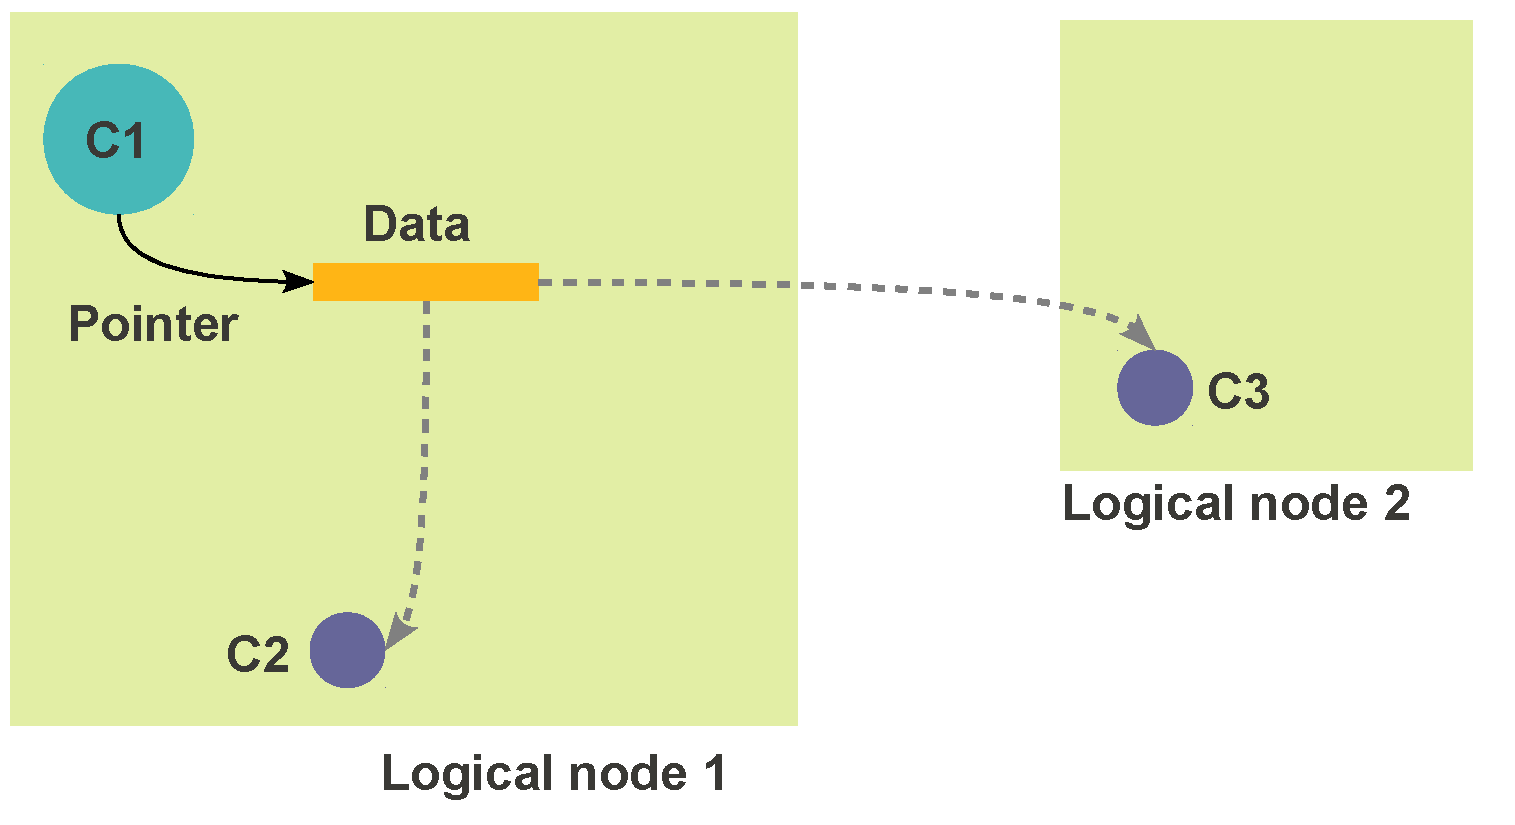
\includegraphics[width=\textwidth]{figures/advancedOpts/fig1}
\end{frame}

\begin{frame}[fragile]
  \begin{itemize}
    \item C1 creates a message that embeds pointer to data
  \end{itemize}
  \frametitle{Conditional packing schematic}
  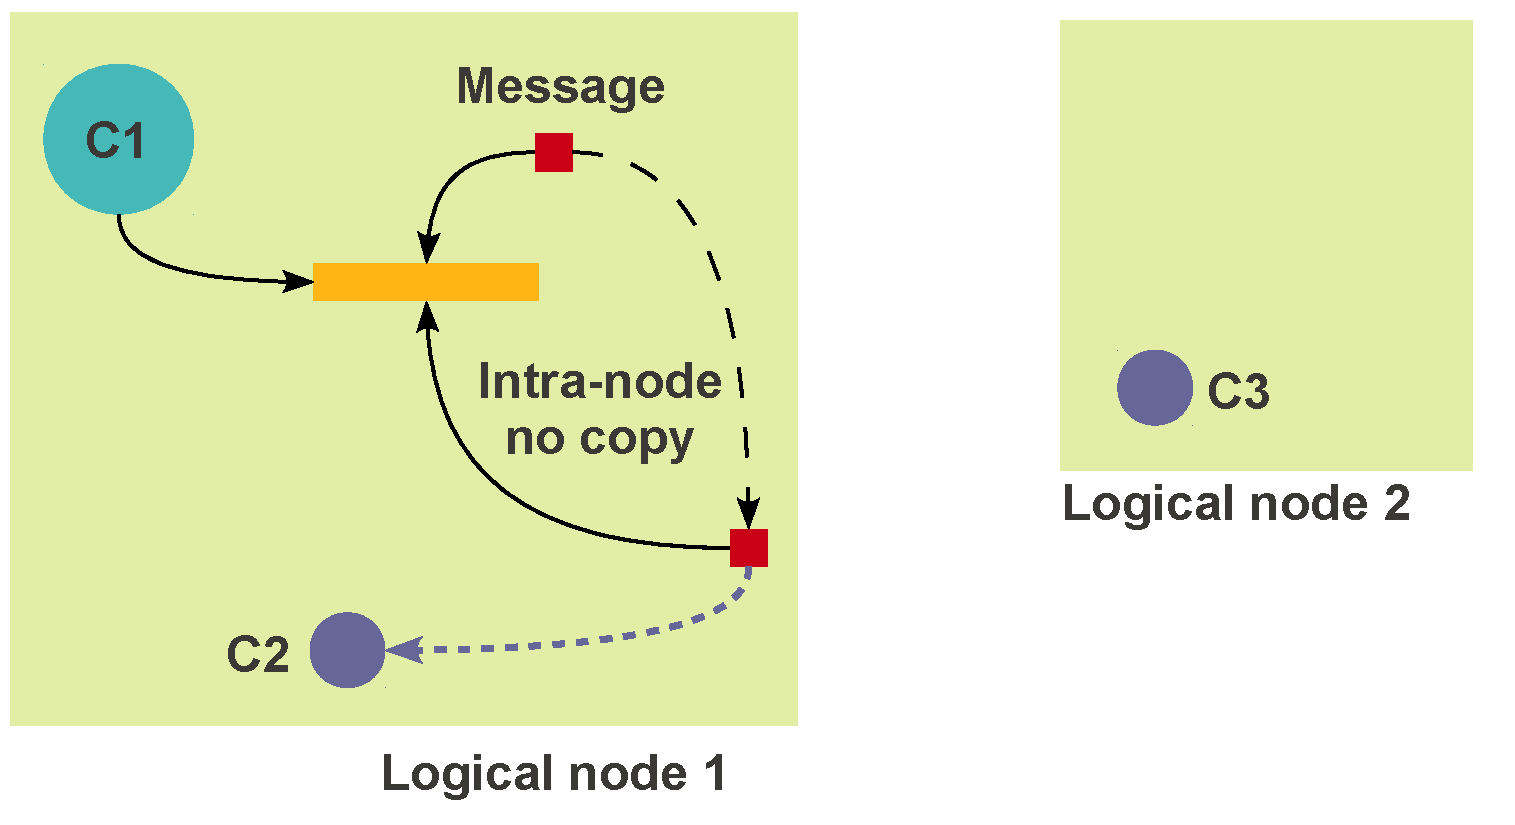
\includegraphics[width=\textwidth]{figures/advancedOpts/fig2}
\end{frame}

\begin{frame}[fragile]
  \begin{itemize}
    \item Message sent to C2 (same node) needs no packing (serialization)
  \end{itemize}
  \frametitle{Conditional packing schematic}
  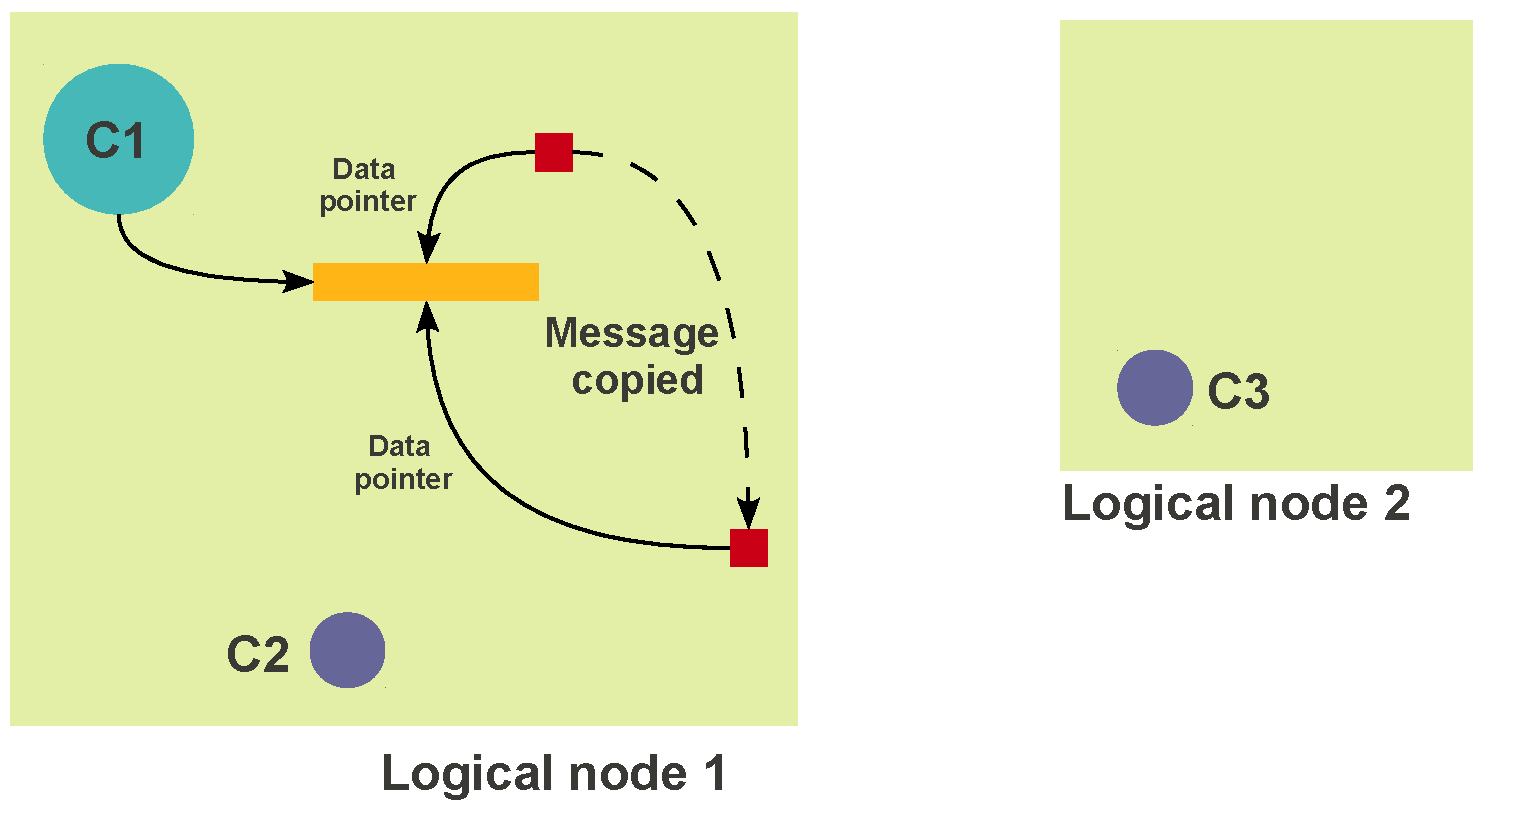
\includegraphics[width=\textwidth]{figures/advancedOpts/fig2_1}
\end{frame}

\begin{frame}[fragile]
  \begin{itemize}
    \item Message processed by C3; uses embedded pointer to access data
  \end{itemize}
  \frametitle{Conditional packing schematic}
  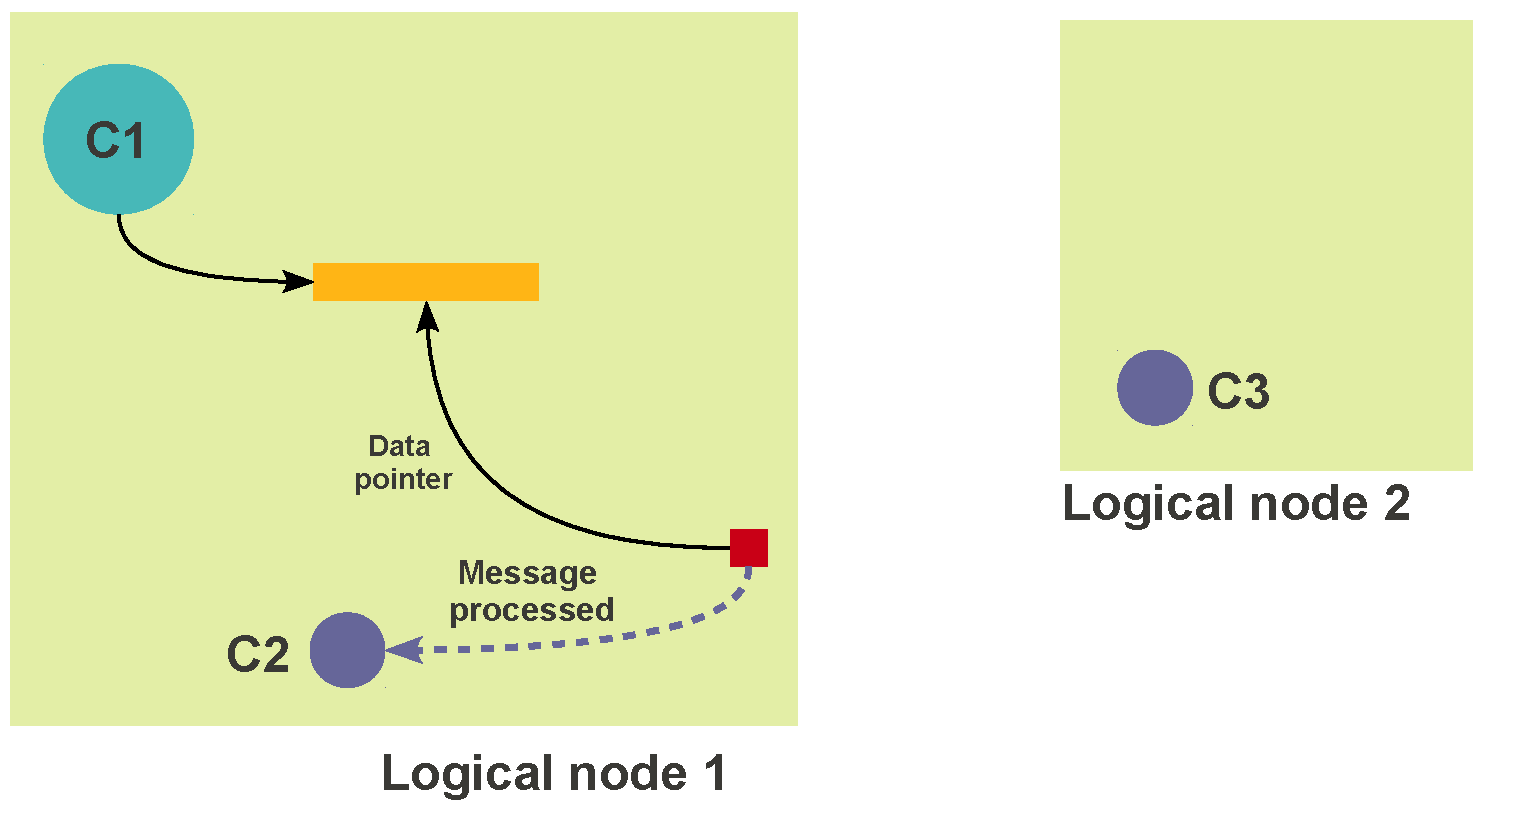
\includegraphics[width=\textwidth]{figures/advancedOpts/fig2_2}
\end{frame}

\begin{frame}[fragile]
  \begin{itemize}
    \item Before sending across node, message is {\em packed}, data serialized
  \end{itemize}
  \frametitle{Conditional packing schematic}
  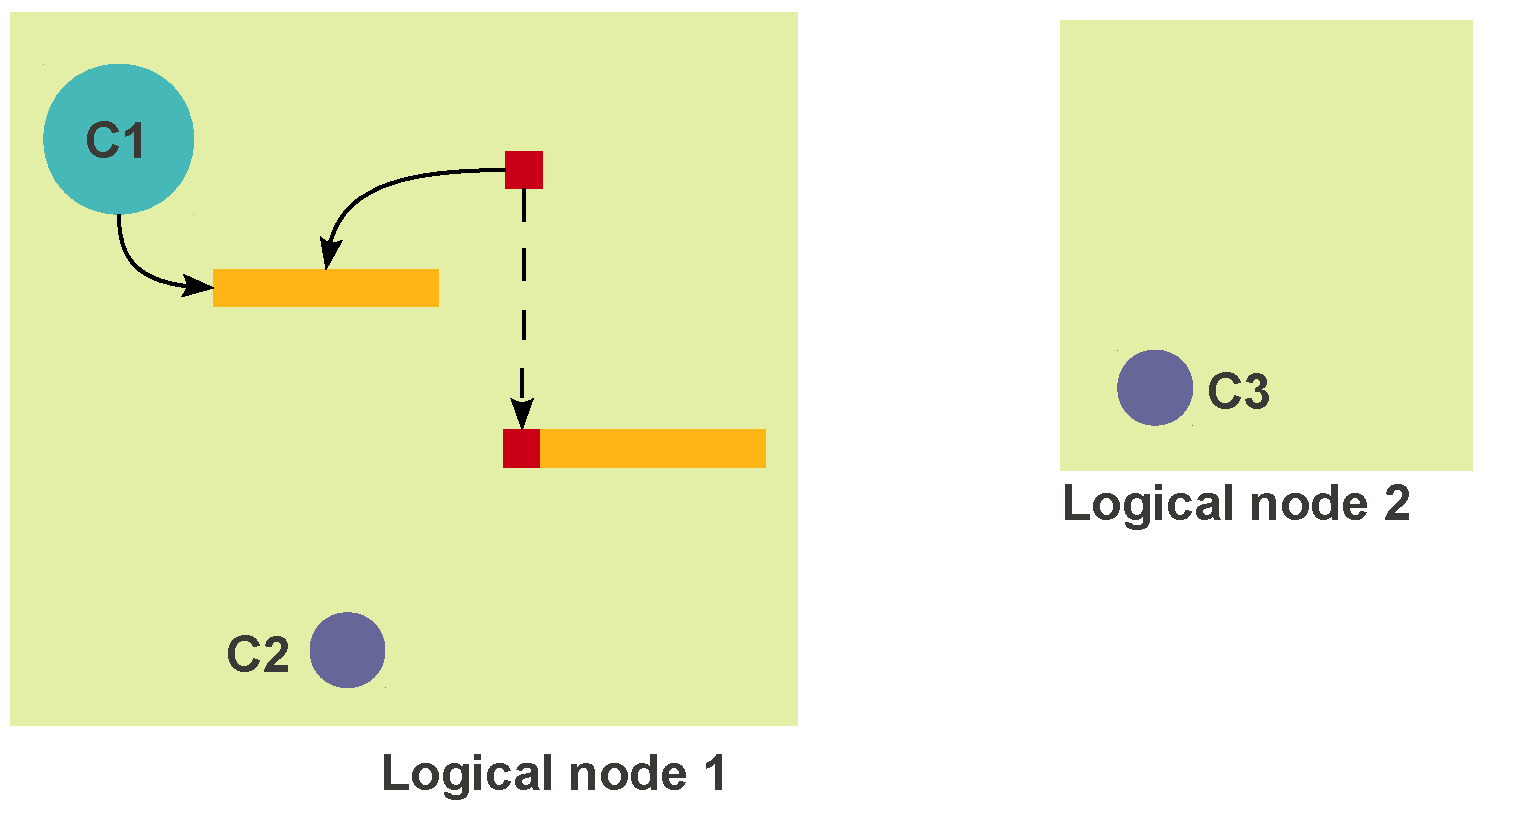
\includegraphics[width=\textwidth]{figures/advancedOpts/fig3}
\end{frame}

\begin{frame}[fragile]
  \frametitle{Conditional packing schematic}
  \begin{itemize}
    \item Message sent over network
  \end{itemize}
  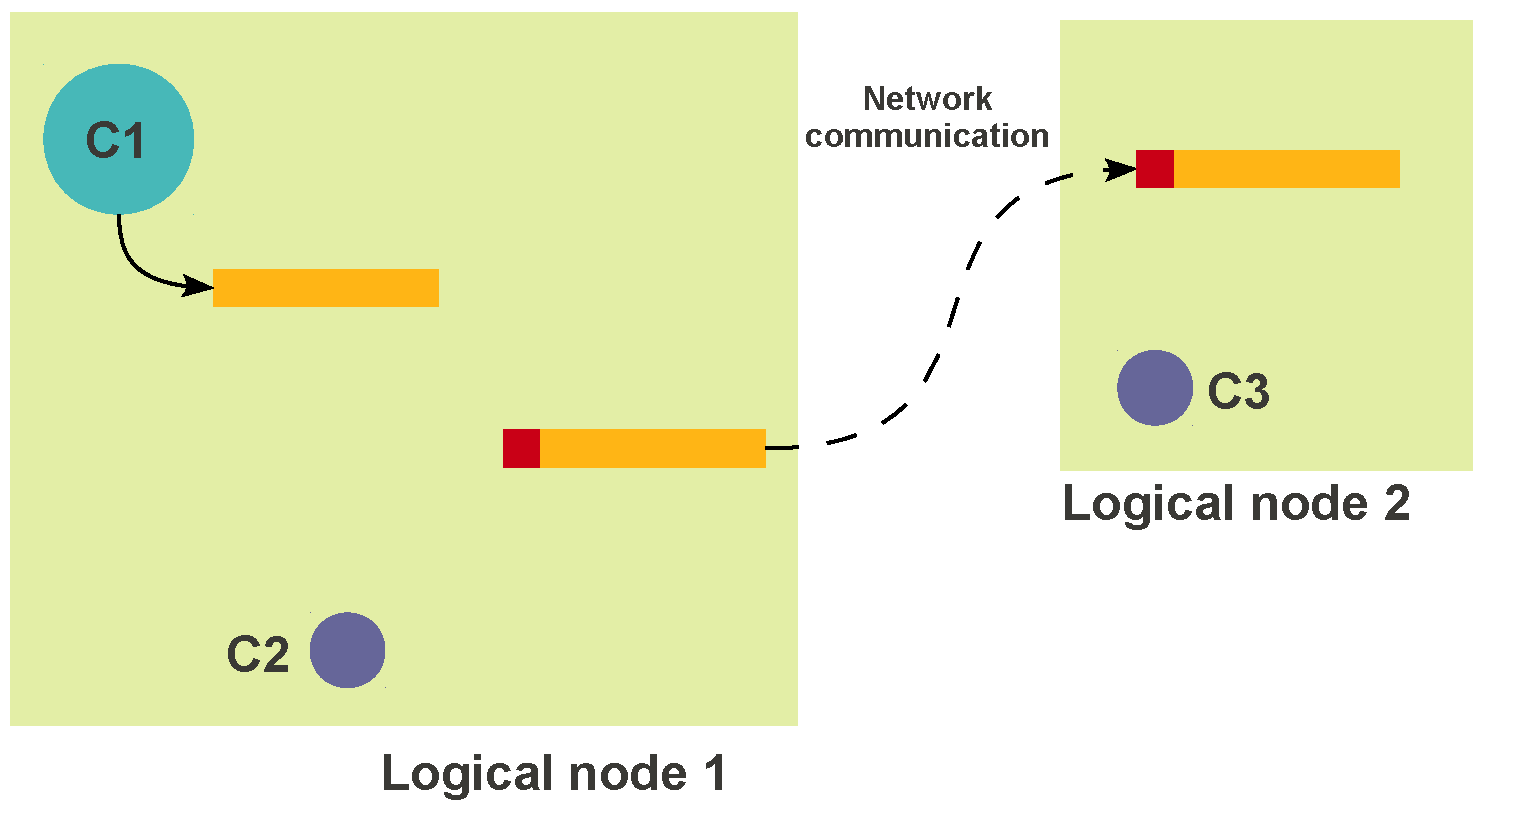
\includegraphics[width=\textwidth]{figures/advancedOpts/fig3_1}
\end{frame}

\begin{frame}[fragile]
  \frametitle{Conditional packing schematic}
  \begin{itemize}
    \item Message {\em unpacked} by Charm++ (calls user-provided function) and processed by C3
  \end{itemize}
  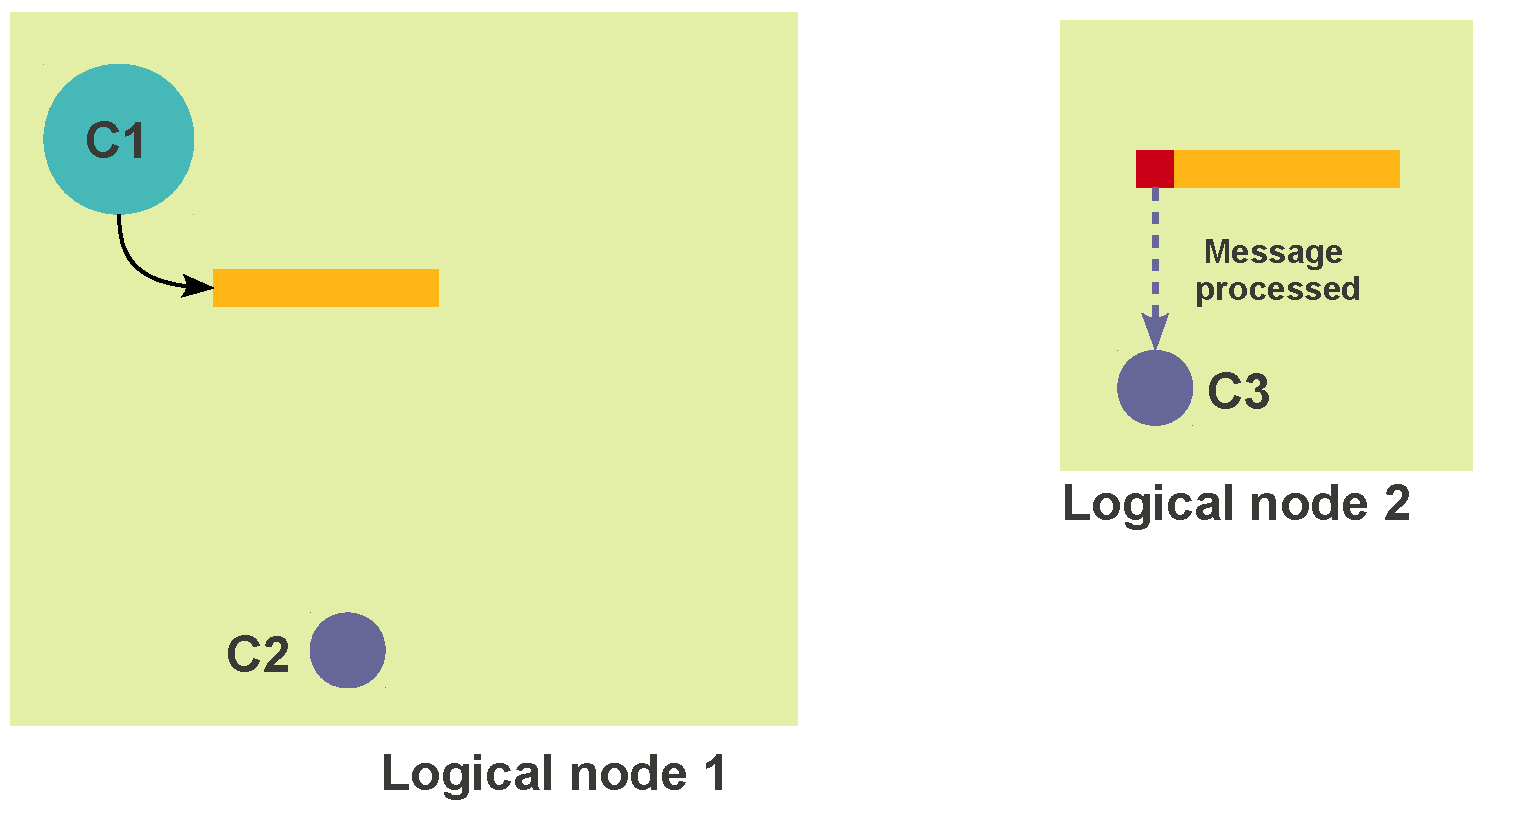
\includegraphics[width=\textwidth]{figures/advancedOpts/fig3_2}
\end{frame}

